


\documentclass[10pt]{article}

\linespread{1} 
\usepackage{float}

\usepackage{geometry}
 \geometry{
  papersize={175mm,248mm},
 total={175mm,248mm},
 left=26mm,
 right=13mm,
 bottom=17mm,
 top=13mm,
 }


\usepackage{amsfonts,amssymb,graphicx,color,epstopdf}
\usepackage[font=small,labelfont=bf]{caption}
\usepackage{subcaption}

\usepackage{color, colortbl, framed}
\usepackage[T1]{fontenc}
\usepackage{mathptmx}

\usepackage{amsmath}
%\usepackage{lineno,hyperref}
\usepackage{authblk}
\usepackage{titlesec}
\usepackage{eucal}
%\DeclareMathAlphabet{\mathpzc}{OT1}{pzc}{m}{it}
%\usepackage{epstopdf}

\usepackage{hhline}
\usepackage{xcolor,colortbl}
\renewcommand{\figurename}{Fig.}

%  \setcounter{secnumdepth}{0}
\usepackage{titlesec}
\titlespacing{\section}{0pt}{\parskip}{-\parskip}
\titlespacing{\subsection}{0pt}{\parskip}{-\parskip}
 \titleformat*{\section}{\normalfont\fontfamily{ptm}\fontsize{10}{19}\bfseries}
 \titleformat*{\subsection}{\normalfont\fontfamily{ptm}\fontsize{10}{18}\bfseries}


\usepackage[sort&compress,square]{natbib}
\setlength{\bibsep}{0.0pt}


\usepackage{authblk}
\usepackage{varwidth}

\renewcommand*{\Authsep}{, }
\renewcommand*{\Authand}{, }
\renewcommand*{\Authands}{, }
\renewcommand*{\Affilfont}{\normalsize\normalfont}
\renewcommand*{\Authfont}{\normalsize\normalfont\bfseries}
\setlength{\affilsep}{0em}

\renewcommand{\abstractname}{}    % clear the title
\makeatletter
\renewcommand{\maketitle}{\bgroup\setlength{\parindent}{0pt}
\begin{flushleft}
  \textbf{\@title}
\vspace{10pt}

  \@author
\end{flushleft}\egroup
}
\makeatother

\title{\fontsize{16pt}{10pt}\selectfont\flushleft \textbf{Informative frequency band identification method using bi-frequency map clustering for fault detection in rotating machines}}

\author[1]{Jacek Wodecki}
\author[2]{Piotr Kruczek}
\author[1]{Justyna Hebda-Sobkowicz}
\author[2]{Agnieszka Wy{\l}oma{\'n}ska}
\author[1]{Radoslaw Zimroz}
\author[3,4]{Konstantinos Gryllias}

\affil[1]{Diagnostics and Vibro-Acoustic Science Laboratory, Wroclaw University of Science and Technology, Na Grobli 15, 50-421 Wroclaw}
\affil[2]{KGHM Cuprum Ltd, Research and Development Centre, Sikorskiego 2-8, 53-659 Wroclaw, Poland}
\affil[3]{Department of Mechanical Engineering, KU Leuven, Celestijnenlaan 300 - box 2420, 3001 Leuven, Belgium}
\affil[4]{Core Lab Dynamics of Mechanical and Mechatronic Systems, Flanders Make, Belgium
\protect\\

\textbf{E-mail:} $^{1}${\{jacek.wodecki, justyna.hebda-sobkowicz, radoslaw.zimroz\}@pwr.edu.pl}, $^{2}${\{pkruczek, awylomanska\}@cuprum.wroc.pl}, $^{3,4}${konstantinos.gryllias@kuleuven.be}}



% \author[label1]{Jacek Wodecki \corref{cor1}}
% \cortext[cor1]{Corresponding author, jacek.wodecki@pwr.edu.pl}
% \author[label2]{Piotr Kruczek}
% \author[label1]{Justyna Hebda-Sobkowicz}
% \author[label2]{Agnieszka Wy{\l}oma{\'n}ska}
% \author[label1]{Radoslaw Zimoz}
% \author[label3]{Konstantinos Gryllias}

% \address[label1]{Diagnostics and Vibro-Acoustic Science Laboratory, Wroclaw University of Science and Technology, Na Grobli 15, 50-421 Wroclaw
% \\\{jacek.wodecki,justyna.hebda-sobkowicz,radoslaw.zimroz\}@pwr.edu.pl\\}
% \address[label2]{KGHM Cuprum Ltd, Research and Development Centre, Sikorskiego 2-8, 53-659 Wroclaw, Poland, \{pkruczek,awylomanska\}@cuprum.wroc.pl\\}
% \address[label3]{Department of Mechanical Engineering, KU Leuven, Celestijnenlaan 300 - box 2420, 3001 Leuven, Belgium, konstantinos.gryllias@kuleuven.be }

\date{} 

\begin{document}
\maketitle
\textbf{Abstract.} In presented work the problem of local damage detection in rolling element bearings is addressed. Usually such issues require the usage of techniques such as decomposition, separation etc. In such real industrial cases the main difficulty lies in the relatively low signal-to-noise ratio as well as at the unpredictable distribution of damage-related information in the frequency domain, hence the typical methods cannot be used. In this paper such an industrial scenario is addressed and a simple yet effective approach to the underlying component extraction is discussed. The proposed method analyzes the Cyclic Spectral Coherence map as the starting data representation and the Expectation-Maximization is used as an analytical tool to determine the Informative Frequency Band (IFB) for impulsive component localization in the carrier frequency spectrum. Finally, based on the identified IFB, the bandpass filter is constructed to extract the impulsive component from the input signal.
\newline \newline
\textbf{Keywords:} Local damage detection, Vibrations, Cyclic Spectral Coherence, Expectation-Maximization.


\section{Introduction}

The area of machine diagnostics is often based on the analysis of vibration signals. In such signals, damage-related information is located in an Informative Frequency Band (IFB) \cite{obuchowski2014selection}. The width, the location and the consistency of the band depends on numerous factors, i.e. the type of damage, the operational conditions, the kinematic structure and the damage location in the machine. In many cases those factors and information about the IFB are not known. Regarding such constraints, it is understandable that research on data-driven methods is a highly pursued direction. Various methods for IFB detection have been proposed over the last years, such as the usage of spectral kurtosis \cite{antoni2009cyclostationarity}, selectors \cite{wylomanska2016impulsive}, the protrugram \cite{barszcz2011novel}, and many others. However, it is very important that not only IFB-related techniques have been successfully developed over recent years. Examples of other directions and approaches include the selective time analysis in time-frequency domain \cite{wodecki2017local}, the multichannel information fusion \cite{wodecki2016combination}, the time-varying filtration \cite{kruczek2017cyclic}, or the heavy-tailed distributions modeling \cite{wylomanska2017application,zak20161932,zak20151731}

In the presented work the authors attempt to determine the IFB based on a bi-frequency map clustering. In this case the modulation spectra vectors are considered as points in the multidimensional feature space and each carrier frequency bin holds a single point. An Expectation-Maximization technique is used to cluster such data, which allows to obtain a precisely bounded IFB. The boundaries of the appropriate cluster are used to design a bandpass filter allowing the extraction of the damage-related impulsive component from the signal.

\section{Methodology}

The proposed procedure consists of three main steps. Firstly the bi-frequency representation of the vibration signal is calculated. In particular the Cyclic Spectral Coherence is used. Secondly the Expectation-Maximization technique is used to cluster individual modulation spectra (for each carrier frequency bin). Finally, the boundaries of the cluster of the CSC map, that can be interpreted as containing the informative frequency band, are used to construct a bandpass filter for impulsive component extraction.

All these techniques are well-known, however their combination is proposed as a successful approach in condition monitoring, focusing specifically on cases, where an impulsive damage-related component investigation is needed but on the other hand a meaningful determination of the IFB is difficult using simpler methods. In this section the definitions and the main properties of the proposed methodology are briefly introduced. Their fusion is illustrated and described afterwards. 

\subsection{Cyclic Spectral Coherence}
The Cyclic Spectral Coherence is a function, which depends on the modulation and the carrier frequency. It has been introduced by Antoni in 2007~\cite{antoni2007cyclic} and it has been proven as a powerful tool to indicate the cyclostationary property of signals. A detailed description of this method can be found in \cite{wodecki2017automatic}.

\subsection{Expectation - Maximization clustering algorithm}
The Expectation -- Maximization (EM) algorithm is an optimization method for the estimation of parameters for given measurement data $X$ \cite{sundberg1974maximum,dempster1977maximum}. EM is especially targeted for separating mixed Gaussian distributions (or any other distribution) in the considered feature space. It is constructed using two main steps which are iterated alternately until achieving the convergence. Clustering in multiple dimensions is the most classic application of this method.

\begin{figure}[ht!]
\centering
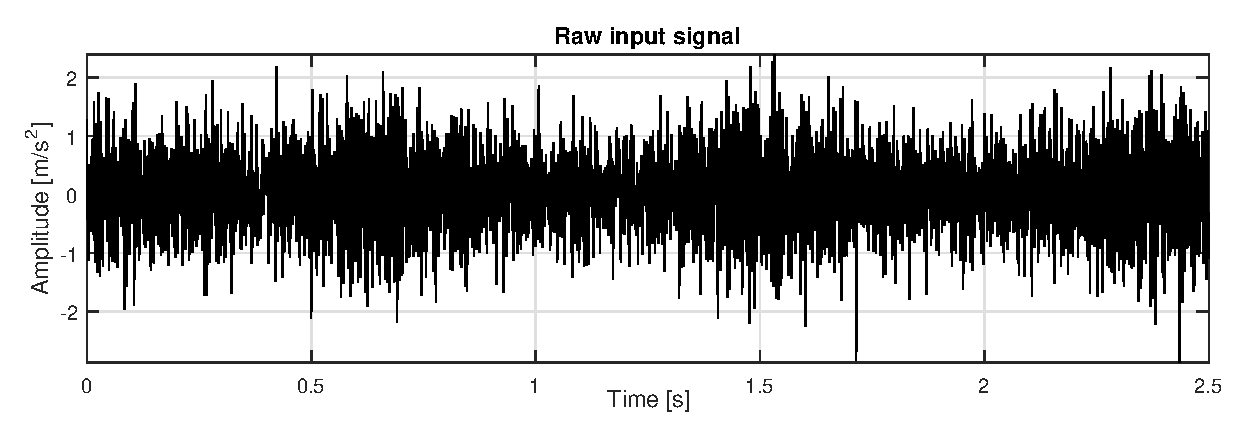
\includegraphics[width=0.7\textwidth]{wykresy/raw.eps}
\caption{Raw input signal}
\label{fig:raw}
\end{figure}
It is very important to be aware of the limitations of the EM methodology. It only approximates the maximum likelihood estimate and does not guarantee finding the theoretical value. If the function of likelihood is not concave, EM does not guarantee to find the global maximum of the function. In practice, it should not be executed only once. Usually one should repeat the EM several times with random initialization and select the one presenting the more effective result. In this paper EM has been run 10 times.

\section{Application to industrial data}
In this article, a vibration signal measured on a rolling bearing is investigated. The bearing is a part of a drive pulley installed in a belt conveyor driving station. The signal is presented in Fig. \ref{fig:raw}. The sampling frequency has been selected equal to 19.2 kHz. The signal contains a single wideband impulsive component corresponding to local damage of the outer race.  The interested readers may find more detailed information regarding this machine to the Ref. \cite{wodecki2018optimal}.

\begin{figure}[ht!]
\centering
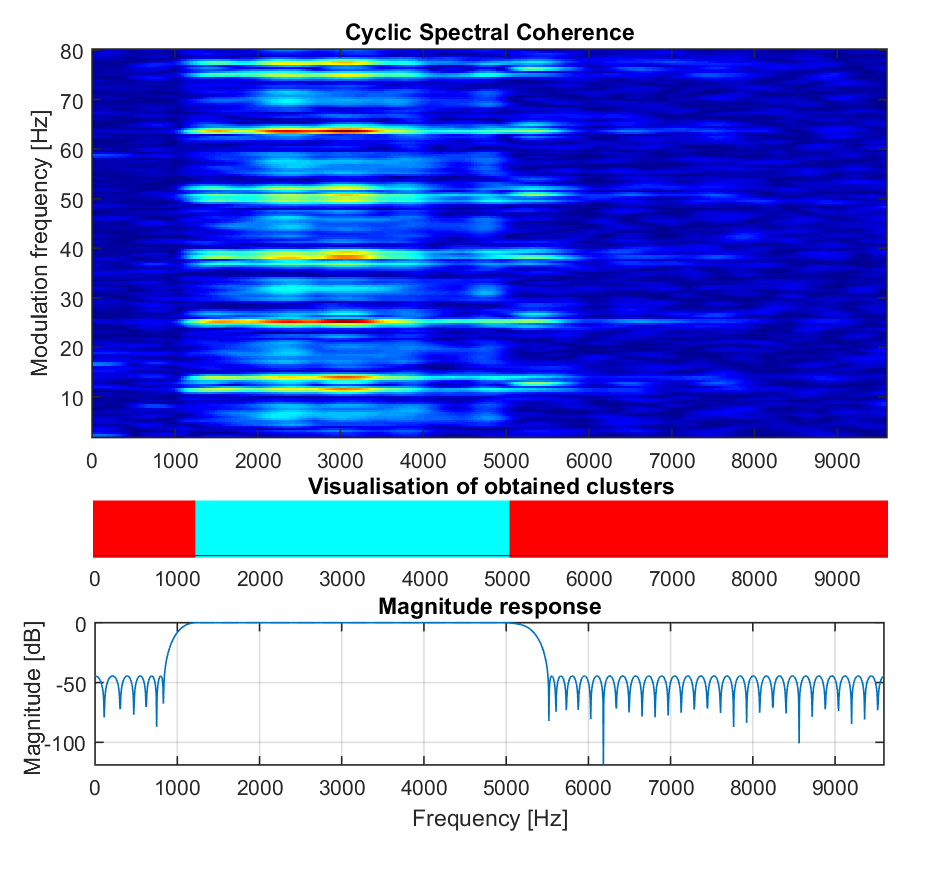
\includegraphics[width=0.8\textwidth]{wykresy/cluster.eps}
\caption{Top: Cyclic Spectral Coherence map of the input signal; Middle: Layout of obtained clusters along the modulating frequency dimension; Bottom: Bandpass filter designed based on obtained clustering results}
\label{fig:cluster}
\end{figure}

The Cyclic Spectral Coherence map of the signal is presented in the top panel of Fig. \ref{fig:cluster}. In the middle panel there is a visual representation of the clustering results, with the carrier frequency axis aligned with the CSC map. EM correctly focuses on the essential part of the carrier frequency band that contains the information about the damage component. The lower and the higher cutoff frequencies of this cluster have been identified equal to 1204 Hz and 5005 Hz respectively. Based on those values, an equiripple bandpass Finite Impulse Response (FIR) filter has been designed using a filter design tool available in Matlab software (see Fig. \ref{fig:cluster} bottom panel).

\begin{figure}[ht!]
\centering
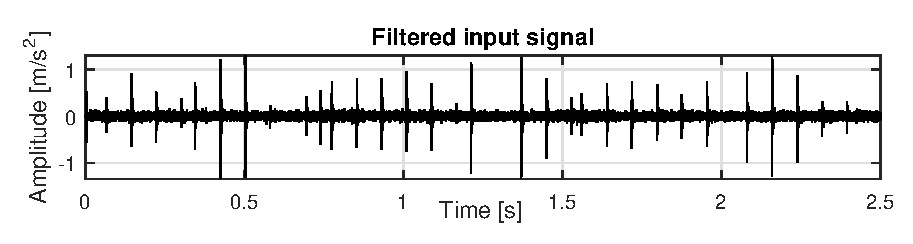
\includegraphics[width=0.9\textwidth]{wykresy/out.eps}
\caption{Extracted damage-related impulsive component}
\label{fig:out}
\end{figure}

The obtained filter has been used to filter the input vibration signal. As a result, the impulsive component has been extracted allowing for a clear and precise observation of damage-related impulsiveness, which is present in the signal. 

\section{Conclusions}

In this paper the authors presented a new method for local damage detection using bi-frequency map clustering for informative frequency band identification, applied to a real vibration signal emitted by a faulty bearing. Instead of using clustering of two-dimensional data representation for recognizing the location of individual impulses in time (in case of using time-frequency maps as a base domain) or in modulating frequency domain (for bi-frequency maps), the Expectation-Maximization algorithm is used in order to identify the Informative Frequency Band on the Cyclic Spectral Coherence map, which is then used to construct the bandpass filter for the processing of the original signal. The results demonstrate the effectiveness of the method to successfully identify the impulsive component of the signal related to the machine fault.

\section*{Acknowledgments}
The work of J.Wodecki and J.Hebda-Sobkowicz was supported by the statutory grant.
\bibliographystyle{style}
\bibliography{mybibfile}

\end{document}